%% USPSC-Apendice.tex
% ---
% Inicia os apêndices
% ---

\begin{apendicesenv}
	% Imprime uma página indicando o início dos apêndices
	\partapendices
	\chapter{Linked Open Social Data for Scientific Benchmarking (diagrams)}\label{ap:losd}

	In this document we provide diagrams
	for the social protocols in the Linked Open Social Database:
	Facebook, Twitter, IRC, Email, ParticipaBR, Cidade Democrática and AA.
	Each social protocol diagram was broken in two, one presents the relations
	among main classes (blue nodes) and data types (orange nodes),
	the other presents metadata for the
	snapshots.
	Every class instance is related to the snapshot instance
	by the triple \textttt{class\_uri po:snapshot snapshot\_uri}.
	Such triples are omitted for simplicity.
	Due to the large number of relations, the rendering of diagrams are
	automatized and displays some overlaps.
	Even so, the images are useful for grasping what is in the current
	database and for conducting explorations.
	Edges in the diagrams have:
	\begin{itemize}
		\item green color if representing an OWL existential
			class restriction (all individuals from the class present at least one triple with
				    the property as predicate);
			    \item inverted nip if representing an OWL universal class
				    restriction (all individuals presenting triples with the
								property as predicate are from the class);
							\item full edges (non-dashed) if representing a functional property
								axiom (there is at most one triple with the property as the
											    predicate for each individual).
	\end{itemize}

	% \textheight = 100pt
	% \pdfpageheight 300pt
	Furthermore, this document ends with two sets of tables, one with
	references for snapshot groups, such as wikipedia or
	contact links, 
	the other with 
	counts of
	triples, participants, edges/interactions/relations and characters.


	\section{Facebook data}
	Each Facebook snapshot is yield by either an user, from which the
	friends constitute a friendship network, or a group, which participants
	can yield friendship and interaction networks and posts information with
	text and some metadata.
	Further information is found on the following diagrams, the tables on
	the end of this document or in the main document of this
	article~\cite{losd}.

	% 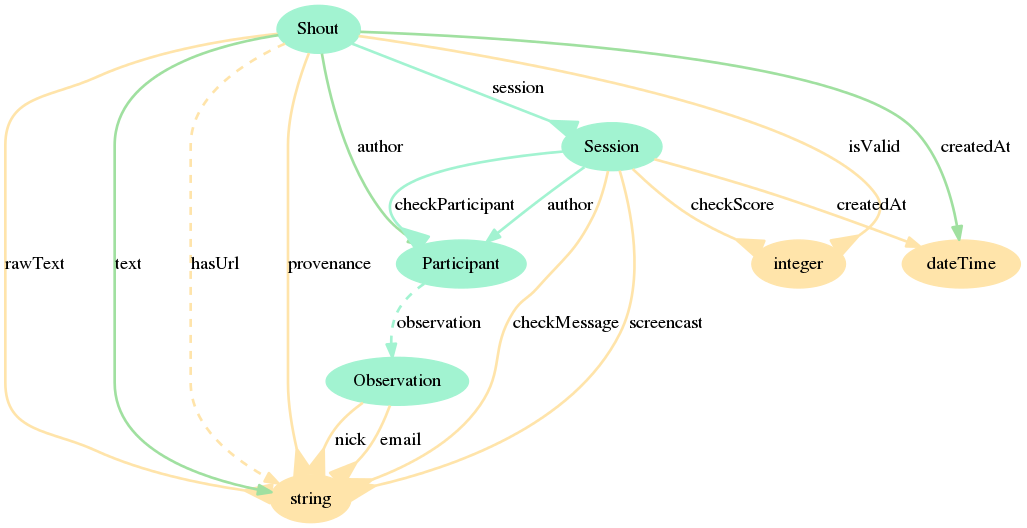
\includepdf{ontologies/aairc.ttl/draw.pdf}
	\incgraph[
		overlay={\node[red,below right] at (page.north west) {\Huge Facebook};}
		      paper=graphics
		      ][scale=.6]{ontologies/facebook-legacy-Auricultura10042013Friendship.ttl/draw.png}

		      \textheight = 2in
		      \pdfpageheight 5in
		      \incgraph[
			      overlay={\node[red,below right] at (page.north west) {\Huge Facebook};}
				    paper=graphics
				    ][scale=.5]{ontologies/facebook-legacy-Auricultura10042013Meta.ttl/draw.png}

				    \section{Twitter data}
				    Each Twitter snapshot is yield by a hashtag.
				    Retweets (\textttt{po:retweetOf} are usually considered the interactions between users.
				    The database present also \textttt{po:replyTo} and \textttt{po:userMention}
				    which might be useful in understanding the networking.
				    Further information is found on the following diagrams, the tables on
				    the end of this document or in the main document of this
				    article~\cite{losd}.

				    \incgraph[
					    overlay={\node[red,below right] at (page.north west) {\Huge
						Twitter };}
						    paper=graphics
						    ][scale=.5]{ontologies/twitter-legacy-arenaNETmundialTweet00000.ttl/draw.png}

						    \incgraph[
							    overlay={\node[red,below right] at (page.north west) {\Huge Twitter};}
								  paper=graphics
								  ][scale=.7]{ontologies/twitter-legacy-arenaNETmundialMeta.ttl/draw.png}

								  \section{IRC data}
								  Each IRC snapshot is yield by an IRC channel.
								  IRC messages are either server messages (e.g. join and exit)
								  marked with \textttt{po:systemMessage true} and having an \textttt{po:impliedUser user\_uri},
								  or user messages, which yield interactions through \textttt{po:directedTo} and \textttt{po:mentions} properties.
								  Text messages without the user names are delivered through the \textttt{po:cleanText} property.
								  Further information is found on the following diagrams, the tables on
								  the end of this document or in the main document of this
								  article~\cite{losd}.
								  \incgraph[
									  overlay={\node[red,below right] at (page.north west) {\Huge IRC};}
										paper=graphics
										][scale=.7]{ontologies/irc-legacy-hackerspace-cpsLog00000.ttl/draw.png}
										\incgraph[
											overlay={\node[red,below right] at (page.north west) {\Huge IRC};}
											      paper=graphics
											      ][scale=.6]{ontologies/irc-legacy-hackerspace-cpsMeta.ttl/draw.png}

											      \section{Email data}
											      Each email snapshot is yield by an Email list.
											      Interactions are yield through \textttt{po:replyTo} relations
											      although \textttt{po:to} and \textttt{po:cc} might also be considered.
											      The email body is given by \textttt{po:text} relations while
											      \textttt{po:cleanText} links to text with lines removed where they are
											      trivially from previous messages or computer code.
											      Further information is found on the following diagrams, the tables on
											      the end of this document or in the main document of this
											      article~\cite{losd}.
											      \incgraph[
												      overlay={\node[red,below right] at (page.north west) {\Huge Email};}
													    paper=graphics
													    ][scale=.4]{ontologies/email-legacy-linux.audio.devel1-20000Email00000.ttl/draw.png}
													    \textheight = 3in
													    \pdfpageheight 6in
													    \incgraph[
														    overlay={\node[red,below right] at (page.north west) {\Huge Email};}
															  paper=graphics
															  ][scale=.5]{ontologies/email-legacy-linux.audio.devel1-20000Meta.ttl/draw.png}

															  \section{ParticipaBR data}
															  The ParticipaBR snapshot is yield by a data dump donated by the system
															  administrators of the federal portal of social participation ParticipaBR.
															  Articles can have parent articles (\textttt{po:parent}), be step of a
															  collection of articles (\textttt{po:stepOf}) and be a mediation of other
															  articles (\textttt{po:mediationOf}).
															  Interactions are yield by comments which are \textttt{po:replyTo} other
															  comments or which are made directly to an article.
															  This snapshot holds also friendship structures.
															  The language used is mainly Brazilian Portuguese, but English and
															  Spanish are also incident.
															  Due to the higher complexity of the diagram, an additional figure is
															  given rendered with another layout algorithm.
															  Further information is found on the following diagrams, the tables on
															  the end of this document or in the main document of this
															  article~\cite{losd}.
															  \incgraph[
																  overlay={\node[red,below right] at (page.north west) {\Huge
																      ParticipaBR};}
																	  paper=graphics
																	  ][scale=.5]{ontologies/participabr.ttl/draw.png}
																	  \incgraph[
																		  overlay={\node[red,below right] at (page.north west) {\Huge
																		      ParticipaBR};}
																			  paper=graphics
																			  ][scale=.7]{ontologies/participabr.ttl/draw_circo.png}
																			  \incgraph[
																				  overlay={\node[red,below right] at (page.north west) {\Huge
																				      ParticipaBR};}
																					  paper=graphics
																					  ][scale=.7]{ontologies/participabrMeta.ttl/draw.png}

																					  \section{Cidade Democrática data}
																					  The Cidade Democrática snapshot is yield by a data dump donated by the system
																					  administrators of the civil society social participation portal Cidade
																					  Democrática.
																					  This snapshot holds a complex structure of both
																					  Topics/Inspirati-ons/Observatories/Supports/Competitions/Prizes
																					  and of State/City/Neighbor-hood/Place.
																					  The language used is mainly Brazilian Portuguese.
																					  Due to the higher complexity of the diagram, an additional figure is
																					  given rendered with another layout algorithm.
																					  Further information is found on the following diagrams, the tables on
																					  the end of this document or in the main document of this
																					  article~\cite{losd}.
																					  \incgraph[
																						  overlay={\node[red,below right] at (page.north west) {\Huge Cidade
																						      Democrática};}
																							  paper=graphics
																							  ][scale=.4]{ontologies/cidadedemocratica00000.ttl/draw.png}
																							  \textheight = 2in
																							  \pdfpageheight 5in
																							  \incgraph[
																								  overlay={\node[red,below right] at (page.north west) {\Huge Cidade
																								      Democrática};}
																									  paper=graphics
																									  ][scale=.4]{ontologies/cidadedemocratica00000.ttl/draw_circo.png}

																									  \incgraph[
																										  overlay={\node[red,below right] at (page.north west) {\Huge Cidade
																										      Democrática};}
																											  paper=graphics
																											  ][scale=.7]{ontologies/cidadedemocraticaMeta.ttl/draw.png}

																											  \section{AA data}
																											  The AA (Algorithmic Autoregulation) snapshots are yield by a data dump donated by the system
																											  administrators and by a mined IRC log.
																											  The system pursue simplicity and most of data consists of detached
																											  shouts with \textttt{po:text} and \textttt{po:author}.
																											  Further information is found on the following diagrams, the tables on
																											  the end of this document or in the main document of this
																											  article~\cite{losd}.
																											  \incgraph[
																												  overlay={\node[red,below right] at (page.north west) {\Huge AA};}
																													paper=graphics
																													][scale=.6]{ontologies/aairc.ttl/draw.png}
																													\textheight = 7in
%																													\pdfpageheight \foobar
																													\incgraph[
																														overlay={\node[red,below right] at (page.north west) {\Huge AA};}
																														      paper=graphics
																														      ][scale=.7]{ontologies/aaircMeta.ttl/draw.png}

																														      \section{Snapshot references}
																														      \label{sreferences}
																														      \pdfpageheight 10in
																														      \begin{table*}[h!]
\begin{center}\scriptsize
\caption{All the Facebook snapshots are either the result of individuals who downloaded
their data (and donated to the first author) or data downloaded from groups.
In the first case, it is senseless to present references. In the second
case, we present the group name and a link to a post in the group where
data and figures were delivered back to the group.}
\begin{tabular}{| l | p{9.9cm} |}\hline
\textbf{group name} & \textbf{url(s)} \\\hline
Adorno Nao Eh Enfeite & \url{https://www.facebook.com/groups/265217103529531/permalink/525654127485826/} \\\hline
Ativistas Da Inclusao Digital & \url{https://www.facebook.com/groups/423602557691243/permalink/525201037531394/} \\\hline
Ciencias Com Fronteiras & \url{https://www.facebook.com/groups/contraaexclusao/permalink/269103356558439/} \\\hline
Computer Art & \url{https://www.facebook.com/groups/computerart/permalink/259389137529870/} \\\hline
Coolmeia &  \url{https://www.facebook.com/groups/coolmeia/permalink/380091142098291/} , \url{https://www.facebook.com/groups/coolmeia/permalink/489757754464962/} \\\hline
Democracia Direta Ja & \url{https://www.facebook.com/groups/ddjbrasil/permalink/347023325397298/} \\\hline
Democracia Pura & \url{https://www.facebook.com/groups/democraciapura/permalink/310907215704321/} \\\hline
Economia & \url{https://www.facebook.com/groups/economa1/permalink/586007714743535/} \\\hline
Economia Criativa Digital & \url{https://www.facebook.com/groups/economiacriativadigital/permalink/438313682916103/} \\\hline
Educacoes E Aprendizagens XXI & \url{https://www.facebook.com/groups/geaxxi/permalink/433229973421182/} \\\hline
Latesfip & \url{https://www.facebook.com/groups/183557128478424/permalink/266610616839741/} \\\hline
Living Bridges Planet & \url{https://www.facebook.com/groups/livingbridgesplanet/permalink/352950408144951/} \\\hline
Mobilizacoes Culturais Interior SP & \url{https://www.facebook.com/groups/131639147005593/permalink/144204529082388/} \\\hline
Partido Pirata & \url{https://www.facebook.com/groups/partidopiratabrasil/permalink/10151409024509317/} \\\hline
Politicas Culturas Brasileiras & \url{https://www.facebook.com/groups/pcult/permalink/519626544747423/} \\\hline
Praca Popular & \url{https://www.facebook.com/groups/215924991863921/permalink/319279541528465/} \\\hline
Rede Tranzmidias & \url{https://www.facebook.com/groups/318333384951196/permalink/346658712118663/} \\\hline
Silicon Valley Global Network & \url{https://www.facebook.com/groups/109971182359978/permalink/589326757757749/} \\\hline
Solidarity Economy & \url{https://www.facebook.com/groups/9149038282/permalink/10151461945623283/} \\\hline
Study Group SNA & \url{https://www.facebook.com/groups/140630009439814/permalink/151470598355755/} \\\hline
Tecnoxamanismo &  \url{https://www.facebook.com/groups/505090906188661/permalink/733144993383250/} , \url{https://www.facebook.com/groups/505090906188661/permalink/733157380048678/} \\\hline
\end{tabular}\end{center}
\end{table*}




																														      \begin{table*}[h!]\scriptsize
																															      \begin{center}
																																      \caption{Different Twitter snapshots are yield by different hashtags. In this
																																      table we present each snapshot with the respective hashtag and a
																																      reference to the subject.}\label{tab:provenance}
																																      \begin{tabular}{| l || p{4cm} | p{4cm} | }\hline
																																	      \textbf{snapshot hashtag} & \textbf{observation} & \textbf{reference} \\\hline\hline
																																		      \#arenaNETmundial & a Brazilian discussion hub about free culture, democracy and the internet & \url{http://www.participa.br/netmundial} \\\hline
																																			  \#art & tweets with the generic hashtag \#art & \url{https://en.wikipedia.org/wiki/Art} \\\hline
																																			      \#ChennaiFloods & heavy rainfall generated by the annual northeast monsoon in November–December 2015 & \url{https://en.wikipedia.org/wiki/2015_South_Indian_floods} \\\hline
																																				  \#dilma & the 36th President of Brazil & \url{https://en.wikipedia.org/wiki/Dilma_Rousseff} \\\hline
																																				      \#ForaDilma & 2015-16 anti-government protests in Brazil & \url{https://en.wikipedia.org/wiki/2015-16_protests_in_Brazil} \\\hline
																																					  \#ForaCunha & 2015-16 anti-corruption protests in Brazil & \url{https://en.wikipedia.org/wiki/2015-16_protests_in_Brazil} \\\hline
																																					      \#fuck & tweets with the generic hashtag \#fuck & \url{https://en.wikipedia.org/wiki/Fuck} \\\hline
																																						  \#game & tweets with the generic hashtag \#game & \url{https://en.wikipedia.org/wiki/Game} \\\hline
																																						      \#god & tweets with the generic hashtag \#god & \url{https://en.wikipedia.org/wiki/God} \\\hline
																																							  \#MAMA2015 & the grand 2015 Mnet Asian Music Awards & \url{https://en.wikipedia.org/wiki/2015_Mnet_Asian_Music_Awards} \\\hline
																																							      \#music & tweets with the generic hashtag \#music & \url{https://en.wikipedia.org/wiki/Music} \\\hline
																																								  \#obama & the 44th President of the United States & \url{https://en.wikipedia.org/wiki/Barack_Obama} \\\hline
																																								      \#python & the Python programming language & \url{https://en.wikipedia.org/wiki/Python_(programming_language)} \\\hline
																																									  \#QuartaSemRacismoClubeSDV & an anti-racism netweaving & \url{https://twitter.com/hashtag/quartasemracismoclubesdv} \\\hline
																																									      \#science & tweets with the generic hashtag \#science & \url{https://en.wikipedia.org/wiki/Science} \\\hline
																																										  \#SnapDetremura & reference for Snapchat about a celebrated person & \url{https://twitter.com/detremura} \\\hline
																																      \end{tabular}\end{center}
																															      \end{table*}                    


																															      \begin{table*}[h!]\scriptsize
																																      \begin{center}
																																	      \caption{Different IRC snapshots are yield by different channels. In this
																																	      table we present each snapshot with the respective channel and a
																																	      reference to the subject.}\label{tab:provenance}
																																	      \begin{tabular}{| l || p{4cm} | p{4cm} | }\hline
																																		      \textbf{snapshot channel} & \textbf{observation} & \textbf{reference} \\\hline\hline
																																			      \#foradoeixo & a Brazilian network of culture related collectives & \url{https://pt.wikipedia.org/wiki/Fora_do_Eixo} \\\hline
																																				  \#hackerspace-cps & a hackerspace in Campinas, Brazil & \url{https://lhc.net.br/wiki/P%C3%A1gina_principal} \\\hline
																																				      \#hackerspaces-br & Brazilian hackerspaces channel & \url{https://garoa.net.br/wiki/Hackerspaces_Brasileiros} \\\hline
																																					  \#labmacambira & Brazilian channel for the labMacambira collective & \url{http://labmacambira.sourceforge.net/} \\\hline
																																	      \end{tabular}\end{center}
																																      \end{table*}                    

																																      \begin{table*}[h!]\scriptsize
																																	      \begin{center}
																																		      \caption{Different Email snapshots are yield by different email lists. In this
																																		      table we present each snapshot with the respective list and a
																																		      reference to the subject.}\label{tab:provenance}
																																		      \begin{tabular}{| p{4cm} || p{4cm} | p{4cm} | }\hline
																																			      \textbf{Gmane ID} & \textbf{observation} & \textbf{reference} \\\hline\hline
																																				      gmane.linux.audio.users & the Linux Audio Users & \url{http://linuxaudio.org} \\\hline
																																					  gmane.politics.organizations.me-tareciclagem & a network about technology and social transformation  & \url{https://metareciclagem.github.io} \\\hline
																																					      gmane.linux.audio.devel & the Linux Audio Developers & \url{http://lists.linuxaudio.org/listinfo/linux-audio-dev} \\\hline
																																						  gmane.comp.gcc.libstdc++.devel & the C++ standard library & \url{https://gcc.gnu.org/libstdc++/} \\\hline
																																		      \end{tabular}\end{center}
																																	      \end{table*}                    

																																	       \begin{table*}[h!]\scriptsize
																																		       \begin{center}
																																			       \caption{References for the snapshots of the detached instances
																																			       ParticipaBR, Cidade Democrática and AA.}\label{tab:provenance}
																																			       \begin{tabular}{| l || p{4cm} | p{3cm} | }\hline
																																				       \textbf{social protocol} & \textbf{observations} & \textbf{reference} \\\hline\hline
																																					       ParticipaBR & a Brazilian federal portal of social participation & \url{http://www.participa.br/} \\\hline
																																						   Cidade Demorática & a Brazilian civil society portal of social participation & \url{http://www.cidadedemocratica.org.br/} \\\hline
																																						       AA & the Algorithmic Autoregulation software development methodology & \cite{aarticle} \\\hline
																																			       \end{tabular}\end{center}
																																		       \end{table*}                    


																																		       \clearpage
																																		       \section{Trivial counts in each snapshot}
																																		       \begin{center}
\scriptsize\begin{longtable}{| l | c | c | c | c |}
\caption{Number of triples (ntriples), number of relations/interactions/edges (nedges), number of participants (nparticipants) and number of characters (nchars) in each snapshot.}
\\
\hline
\textbf{snapshot id} & \textbf{ntriples}  & \textbf{nedges}  & \textbf{nparticipants}  & \textbf{nchars} \\\hline\hline
\endfirsthead
\multicolumn{5}{c}{\tablename\ \thetable\ -- \textit{Continued from previous page}} \\\hline
\textbf{snapshot id} & \textbf{ntriples}  & \textbf{nedges}  & \textbf{nparticipants}  & \textbf{nchars} \\\hline\hline\endhead
\multicolumn{5}{r}{\textit{Continued on next page}} \\
\endfoot\endlastfoot

aa-irc-legacy-labmacambira\_lalenia.txt & 53,140  & 0  & 117  & 558,466 \\\hline
aa-mongo-legacy & 22,773  & 0  & 37  & 240,172 \\\hline
aa-mysql-legacy & 790,796  & 0  & 157  & 2,753,354 \\\hline
cidadedemocratica-legacy & 915,852  & 0  & 23,079  & 6,871,848 \\\hline
facebook-legacy-AdornoNaoEhEnfeite29032013 & 8,459  & 1,292  & 293  & 26,113 \\\hline
facebook-legacy-AntonioAnzoategui18022013 & 1,676  & 328  & 52  & 0 \\\hline
facebook-legacy-AtivistasDaInclusaoDigital09032013 & 25,642  & 5,592  & 306  & 0 \\\hline
facebook-legacy-Auricultura10042013 & 19,515  & 3,898  & 412  & 14,015 \\\hline
facebook-legacy-BrunoMialich31012013 & 40,794  & 9,320  & 502  & 0 \\\hline
facebook-legacy-CalebLuporini13042013 & 105,962  & 24,653  & 1,050  & 0 \\\hline
facebook-legacy-CalebLuporini19022013 & 104,746  & 24,391  & 1,026  & 0 \\\hline
facebook-legacy-CienciasComFronteiras29032013 & 110,734  & 23,302  & 2,921  & 0 \\\hline
facebook-legacy-ComputerArt10032013 & 260,050  & 62,819  & 1,342  & 0 \\\hline
facebook-legacy-Coolmeia06032013 & 76,063  & 16,534  & 1,202  & 0 \\\hline
facebook-legacy-DanielPenalva18022013 & 3,519  & 682  & 113  & 0 \\\hline
facebook-legacy-DemocraciaDiretaJa14032013 & 258,679  & 59,323  & 3,053  & 54,443 \\\hline
facebook-legacy-DemocraciaDiretaJa14072013 & 257,490  & 59,781  & 3,607  & 58,035 \\\hline
facebook-legacy-DemocraciaPura06042013 & 32,227  & 6,730  & 627  & 65,062 \\\hline
facebook-legacy-Economia14042013 & 238,790  & 54,001  & 3,587  & 52,664 \\\hline
facebook-legacy-EconomiaCriativaDigital03032013 & 185,905  & 43,128  & 1,684  & 0 \\\hline
facebook-legacy-EducacoesEAprendizagensXXI02032013 & 106,918  & 24,802  & 1,285  & 0 \\\hline
facebook-legacy-GabrielaThume19022013 & 18,581  & 4,108  & 307  & 0 \\\hline
facebook-legacy-GrahamForrest28012013 & 1,370  & 185  & 90  & 0 \\\hline
facebook-legacy-LailaManuelle17012013 & 201,071  & 48,572  & 969  & 0 \\\hline
facebook-legacy-LarissaAnzoategui20022013 & 24,824  & 5,191  & 580  & 0 \\\hline
facebook-legacy-Latesfip08032014 & 11,554  & 2,009  & 306  & 0 \\\hline
facebook-legacy-LivingBridgesPlanet29032013 & 149,708  & 32,494  & 3,077  & 52,808 \\\hline
facebook-legacy-LuisCirne07032013 & 16,619  & 3,390  & 437  & 0 \\\hline
facebook-legacy-MariliaMelloPisani10042013 & 84,770  & 19,040  & 1,230  & 0 \\\hline
facebook-legacy-Mirtes16052013 & 39,415  & 9,075  & 445  & 0 \\\hline
facebook-legacy-MobilizacoesCulturaisInteriorSP13032013 & 26,518  & 6,096  & 298  & 0 \\\hline
facebook-legacy-PartidoPirata23032013 & 45,495  & 8,537  & 1,943  & 36,313 \\\hline
facebook-legacy-PedroPauloRocha10032013 & 215,888  & 50,591  & 1,932  & 0 \\\hline
facebook-legacy-PeterForrest28012013 & 8,156  & 1,829  & 120  & 0 \\\hline
facebook-legacy-PoliticasCulturasBrasileiras08032013 & 178,289  & 41,690  & 1,278  & 69,756 \\\hline
facebook-legacy-PracaPopular16032013 & 4,539  & 932  & 65  & 4,249 \\\hline
facebook-legacy-RafaelReinehr09042013 & 174,423  & 39,586  & 2,297  & 0 \\\hline
facebook-legacy-RamiroGiroldo20022013 & 9,928  & 2,020  & 264  & 0 \\\hline
facebook-legacy-RedeTranzmidias02032013 & 25,111  & 4,940  & 391  & 54,907 \\\hline
facebook-legacy-RenatoFabbri02032013 & 93,134  & 21,579  & 974  & 0 \\\hline
facebook-legacy-RenatoFabbri03032013 & 93,690  & 21,711  & 978  & 0 \\\hline
facebook-legacy-RenatoFabbri11072013 & 114,552  & 26,440  & 1,256  & 0 \\\hline
facebook-legacy-RenatoFabbri18042013 & 104,156  & 24,072  & 1,124  & 0 \\\hline
facebook-legacy-RenatoFabbri20012013 & 86,416  & 20,085  & 868  & 0 \\\hline
facebook-legacy-RenatoFabbri29112012 & 82,093  & 19,083  & 823  & 0 \\\hline
facebook-legacy-RicardoFabbri18022013 & 11,372  & 2,327  & 344  & 0 \\\hline
facebook-legacy-RitaWu08042013 & 83,895  & 18,935  & 1,165  & 0 \\\hline
facebook-legacy-RonaldCosta12062013 & 31,338  & 6,557  & 730  & 0 \\\hline
facebook-legacy-SiliconValleyGlobalNetwork27042013 & 77,158  & 15,740  & 2,130  & 50,251 \\\hline
facebook-legacy-SolidarityEconomy12042013 & 14,230  & 2,404  & 525  & 67,774 \\\hline
facebook-legacy-StudyGroupSNA05042013 & 5,604  & 480  & 448  & 25,474 \\\hline
facebook-legacy-THackDay26032013 & 1,844  & 420  & 41  & 0 \\\hline
facebook-legacy-Tecnoxamanismo08032014 & 11,106  & 2,069  & 318  & 0 \\\hline
facebook-legacy-Tecnoxamanismo15032014 & 14,589  & 2,702  & 450  & 0 \\\hline
facebook-legacy-ThaisTeixeira19022013 & 26,424  & 6,088  & 296  & 0 \\\hline
facebook-legacy-VilsonVieira18022013 & 19,688  & 4,334  & 336  & 0 \\\hline
facebook-legacy-ViniciusSampaio18022013 & 90,515  & 21,360  & 725  & 0 \\\hline
facebook-legacy-avlab\_BarthorLaZule22022014 & 16,005  & 3,513  & 279  & 0 \\\hline
facebook-legacy-avlab\_CalebLuporini25022014 & 125,577  & 29,268  & 1,215  & 0 \\\hline
facebook-legacy-avlab\_CamilaBatista23022014 & 21,138  & 4,476  & 462  & 0 \\\hline
facebook-legacy-avlab\_CarlosDiego25022014 & 171,744  & 39,401  & 2,020  & 0 \\\hline
facebook-legacy-avlab\_CristinaMekitarian23022014 & 24,647  & 5,572  & 337  & 0 \\\hline
facebook-legacy-avlab\_DanielGonzales23022014 & 196,406  & 45,318  & 2,162  & 0 \\\hline
facebook-legacy-avlab\_FelipeBrait23022014 & 1,228,605  & 299,082  & 4,611  & 0 \\\hline
facebook-legacy-avlab\_FelipeVillela22022014 & 2,475  & 477  & 81  & 0 \\\hline
facebook-legacy-avlab\_JoaoMeirelles25022014 & 52,371  & 11,649  & 825  & 0 \\\hline
facebook-legacy-avlab\_JoaoMekitarian23022014 & 88,765  & 20,821  & 783  & 0 \\\hline
facebook-legacy-avlab\_JulianaSouza23022014 & 129,757  & 29,942  & 1,427  & 0 \\\hline
facebook-legacy-avlab\_KarinaGomes22022014 & 9,073  & 1,906  & 207  & 0 \\\hline
facebook-legacy-avlab\_LucasOliveira26022014 & 62,871  & 14,764  & 545  & 0 \\\hline
facebook-legacy-avlab\_MarcelaLucatelli25022014 & 138,733  & 31,647  & 1,735  & 0 \\\hline
facebook-legacy-avlab\_MariliaPisani25022014 & 114,765  & 25,830  & 1,635  & 0 \\\hline
facebook-legacy-avlab\_NatachaRena22022014 & 642,769  & 154,758  & 3,391  & 0 \\\hline
facebook-legacy-avlab\_OrlandoCoelho22022014 & 5,149  & 848  & 251  & 0 \\\hline
facebook-legacy-avlab\_PalomaKliss25022014 & 493,774  & 119,520  & 2,242  & 0 \\\hline
facebook-legacy-avlab\_PedroRocha25022014 & 346,883  & 81,910  & 2,749  & 0 \\\hline
facebook-legacy-avlab\_RenatoFabbri22022014 & 124,703  & 28,780  & 1,369  & 0 \\\hline
facebook-legacy-avlab\_SarahLuporini25022014 & 505,853  & 121,502  & 2,835  & 0 \\\hline
facebook-legacy-avlab\_SatoBrasil25022014 & 1,519,394  & 371,249  & 4,914  & 0 \\\hline
facebook-legacy-ego\_MarceloSaldanha19112014 & 130,556  & 29,440  & 1,828  & 0 \\\hline
facebook-legacy-ego\_MariliaPisani06052014 & 122,231  & 27,581  & 1,701  & 0 \\\hline
facebook-legacy-ego\_MassimoCanevacci19062013 & 273,328  & 59,995  & 4,764  & 0 \\\hline
facebook-legacy-ego\_RenatoFabbri06022014 & 123,993  & 28,606  & 1,367  & 0 \\\hline
facebook-legacy-ego\_RenatoFabbri19112014 & 153,410  & 35,514  & 1,622  & 0 \\\hline
facebook-legacy-ego\_VJPixel23052014 & 231,608  & 54,752  & 1,800  & 0 \\\hline
facebook-legacy-posavlab\_AnaCelia18032014 & 53,939  & 12,167  & 753  & 0 \\\hline
facebook-legacy-posavlab\_ElenaGarnelo04032014 & 93,472  & 21,723  & 940  & 0 \\\hline
facebook-legacy-posavlab\_FabiBorges08032014 & 159,584  & 36,592  & 1,888  & 0 \\\hline
facebook-legacy-posavlab\_GeorgeSanders08032014 & 108,071  & 24,706  & 1,321  & 0 \\\hline
facebook-legacy-posavlab\_GrazielleMachado18032014 & 24,264  & 5,254  & 464  & 0 \\\hline
facebook-legacy-posavlab\_RenatoFabbri19032014 & 129,360  & 29,890  & 1,400  & 0 \\\hline
facebook-legacy-posavlab\_RicardoPoppi18032014 & 76,104  & 17,234  & 1,024  & 0 \\\hline
gmane-legacy-comp.gcc.libstdcpp.devel1-20000 & 324,051  & 14,786  & 1,036  & 30,126,252 \\\hline
gmane-legacy-linux.audio.devel1-20000 & 377,307  & 17,076  & 1,232  & 26,969,596 \\\hline
gmane-legacy-linux.audio.users1-20000 & 349,304  & 16,362  & 1,147  & 25,065,928 \\\hline
gmane-legacy-politics.organizations.metareciclagem1-20000 & 338,679  & 15,230  & 477  & 54,260,954 \\\hline
irc-legacy-foradoeixo & 685,623  & 4,308  & 3,318  & 3,777,424 \\\hline
irc-legacy-hackerspace-cps & 253,614  & 1,860  & 607  & 1,059,675 \\\hline
irc-legacy-hackerspaces-br & 980,556  & 210  & 347  & 8,420,840 \\\hline
irc-legacy-labmacambira & 1,535,463  & 58,525  & 1,561  & 8,358,970 \\\hline
participabr-legacy & 159,602  & 2,207  & 3,825  & 2,045,617 \\\hline
twitter-legacy-ChennaiFloods & 6,793,705  & 101,824  & 46,493  & 23,237,802 \\\hline
twitter-legacy-ForaCunha & 88,963  & 1,656  & 2,747  & 372,131 \\\hline
twitter-legacy-ForaDilma & 26,818  & 668  & 659  & 113,810 \\\hline
twitter-legacy-MAMA2015 & 20,356,960  & 426,558  & 33,080  & 75,358,785 \\\hline
twitter-legacy-QuartaSemRacismoClubeSDV & 367,460  & 5,000  & 5,785  & 1,635,867 \\\hline
twitter-legacy-SnapDetremura & 26,834  & 461  & 621  & 124,448 \\\hline
twitter-legacy-arenaNETmundial & 388,134  & 15,797  & 5,898  & 2,825,121 \\\hline
twitter-legacy-art & 2,814,803  & 32,655  & 30,486  & 9,539,413 \\\hline
twitter-legacy-dilma & 78,424  & 1,692  & 2,274  & 332,005 \\\hline
twitter-legacy-fuck & 3,631  & 40  & 93  & 14,727 \\\hline
twitter-legacy-game & 229,992  & 1,548  & 4,682  & 1,229,910 \\\hline
twitter-legacy-god & 1,514,365  & 20,132  & 22,117  & 5,560,140 \\\hline
twitter-legacy-music & 8,150,863  & 39,456  & 54,006  & 21,116,573 \\\hline
twitter-legacy-obama & 1,143,873  & 20,623  & 20,330  & 4,481,840 \\\hline
twitter-legacy-python & 5,786  & 4  & 17  & 1,758 \\\hline
twitter-legacy-science & 369,013  & 3,673  & 7,156  & 1,910,216 \\\hline
\end{longtable}
\end{center}







																																	       \end{apendicesenv}
																																	       % ---
